
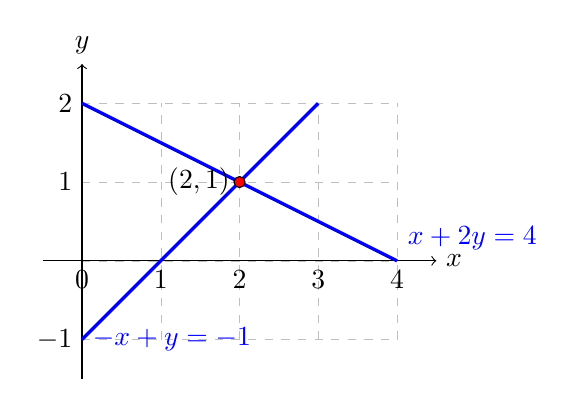
\begin{tikzpicture}
    \draw[step=1,help lines, dashed,lightgray] (0,-1) grid (4,2);
    %draw axis value
    \foreach \x in {0,1,2,3,4}
        {%
            \draw (\x,0) -- (\x,0) node [below] {$\x$};
        }
    \foreach \y in {-1,1,2}
        {%
            \draw (0,\y) -- (0,\y) node [left] {$\y$};
        }
    %draw lines
    \draw [->] (-0.5,0) -- (4.5,0) node[right]{$x$};
    \draw [->] (0,-1.5) -- (0,2.5) node[above]{$y$};
    \draw [-,blue,very thick]  (0,2) -- (4,0) node[above right]{$x+2y=4$};
    \draw [-,blue,very thick]  (3,2) -- (0,-1) node[right]{$-x+y=-1$};
    \draw [fill=red] (2,1) circle[radius=2pt] node[left]{$(2,1)$};
\end{tikzpicture}
\captionof{figure}{{\footnotesize 2D vector, $\vec{v}=(3,2)\in{R^2}$}}
\label{fig:linear-system-and-subspaces-d1}
